\documentclass[a4paper,11pt]{article}
\usepackage{sbpo-template}
\usepackage[brazil]{babel}    % português do Brasil
\usepackage[utf8]{inputenc}   % acentos no UTF-8
\usepackage[T1]{fontenc}      % para hifenização correta
\usepackage{amsmath,amssymb}
\usepackage{url}
\usepackage[square]{natbib}
\usepackage{indentfirst}
\usepackage{fancyhdr}
\usepackage{graphicx}
\usepackage{booktabs}
\pagestyle{fancy}
\fancyhf{}
\fancyhead[C]{
\includegraphics[scale=0.5]{sbpo2026-header-logo.png}}
\renewcommand{\headruleskip}{-1mm}
\setlength\headheight{86pt}
\addtolength{\textheight}{-86pt}
\setlength{\headsep}{5mm}
\setlength{\footskip}{4.08003pt}

\begin{document}

\title{xR --- Recuperação Esperada sob Pressão: um modelo logístico calibrado com alvo espacialmente restrito para análise tática no futebol}

\maketitle
\thispagestyle{fancy}

% ===== ESPAÇO PARA 3 AUTORES (preencher / remover para submissão cega) =====
\author{
\name{Primeiro Autor}
\institute{Filiação}
\iaddress{Endereço da Instituição}
\email{e-mail}
}

\author{
\name{Segundo Autor}
\institute{Filiação}
\iaddress{Endereço da Instituição}
\email{e-mail}
}

\author{
\name{Terceiro Autor}
\institute{Filiação}
\iaddress{Endereço da Instituição}
\email{e-mail}
}

\vspace{8mm}
\begin{resumo}
Avaliar se um jogador deveria ou não perder a posse sob pressão é central na análise tática do futebol. Propomos o \emph{xR} (Recuperação Esperada), a probabilidade calibrada de a equipe que pressiona recuperar a bola, estimada a partir do StatsBomb-360. Mostramos empiricamente que a \textbf{definição do alvo} --- e não a arquitetura do modelo --- é a principal alavanca preditiva: restringir o sucesso no tempo e no espaço (recuperar em até 5\,s e a até 5\,m) eleva a AUC de 0,59 para 0,70, enquanto GNN, CNN e Set Transformer, \emph{sob o alvo padrão de recuperação em até 10\,s}, estacionam em $\approx$0,59. Uma regressão logística \textbf{leve e calibrada} (ECE 0,003) iguala modelos pesados e habilita usos agregados: análise de adversário, treino, \emph{scouting} e revisão pós-jogo (xR \emph{vs.} realizado). Delimitamos honestamente o escopo: \emph{ratings} individuais de jogador têm confiabilidade $\approx$0,09, inadequados para veredito individual.
\end{resumo}

\bigskip
\begin{palchaves}
Análise esportiva, Aprendizado de máquina, Modelos calibrados.

\bigskip
\noindent{Tópicos: EST -- Estatística; ADA -- Análise de Dados; Aplicações em Esporte.}
\end{palchaves}

\vspace{8mm}

\begin{abstract}
Assessing whether a player should or should not lose possession under pressure is central to tactical football analysis. We propose \emph{xR} (Expected Recovery), the calibrated probability that the pressing team regains the ball, estimated from StatsBomb-360 data. We show empirically that the \textbf{target definition} --- not the model architecture --- is the main predictive lever: constraining success in time and space (recovery within 5\,s and 5\,m) raises AUC from 0.59 to 0.70, while GNN, CNN and Set Transformer plateau at $\approx$0.59 \emph{under the standard 10\,s recovery target}. A \textbf{light, calibrated} logistic regression (ECE 0.003) matches heavy models and enables aggregate uses: opponent analysis, training, scouting and post-match review (xR \emph{vs.} actual). We honestly delimit scope: individual player ratings have reliability $\approx$0.09, unfit for individual verdicts.
\end{abstract}

\bigskip
\begin{keywords}
Sports analytics, Machine learning, Calibrated models.

\bigskip
\noindent{Paper topics: Statistics; Data Analysis; Sports Applications.}
\end{keywords}

\newpage
\section{Introdução}

O \emph{pressing} --- a pressão coordenada sobre o portador da bola e seus arredores --- tornou-se um pilar tático do futebol de elite. Quantificar sua eficácia, e em particular avaliar \textbf{se um jogador deveria ou não perder a posse} em um contexto específico, é de interesse direto para comissões técnicas, no treino, na análise de adversário e no \emph{scouting}. A literatura recente ataca o problema com dados de eventos e, mais recentemente, dados posicionais \citep{robberechts2019,merckx2021,lee2025express}, mas duas lacunas persistem: (i) os modelos preditivos estacionam em desempenho modesto (AUC $\approx$ 0,60), sem uma explicação clara do porquê; e (ii) os \emph{ratings} individuais de jogador são apresentados de forma anedótica, sem auditoria de confiabilidade.

Este trabalho propõe o \textbf{xR (Recuperação Esperada)}: a probabilidade calibrada de a equipe que pressiona recuperar a bola dentro de uma janela curta, vista do lado do portador como o risco de \emph{perder} a posse. A partir de uma extensa jornada experimental sobre o StatsBomb Open Data (incluindo a UEFA Euro 2020 e a Copa do Mundo FIFA 2022), nossas contribuições são:

\begin{enumerate}
\item \textbf{Achado central (o alvo define o sinal).} Mostramos, por ablação, que a informatividade da geometria dos jogadores depende de \emph{como} se define o sucesso do pressing. Restringir o desfecho no tempo \emph{e} no espaço (recuperar em $\le$5\,s e a $\le$5\,m do ponto de pressão) eleva a AUC de 0,59 para 0,70 com as \emph{mesmas} variáveis, enquanto arquiteturas profundas (GNN, CNN, Set Transformer) não ultrapassam $\approx$0,59 sob o alvo padrão de recuperação em $\le$10\,s.
\item \textbf{Um modelo proposto leve e calibrado.} Uma regressão logística sobre atributos geométricos, com o alvo espacialmente restrito, iguala modelos pesados na qualidade probabilística (ECE 0,003) e é interpretável --- adequada para uso por analistas e comissão técnica.
\item \textbf{Delimitação honesta de escopo.} Quantificamos a confiabilidade dos \emph{ratings} individuais de jogador ($\approx$0,09 mesmo com 91.692 pressões), mostrando que o modelo é uma ferramenta \emph{agregada} de apoio à decisão, não um juiz de jogadas ou de jogadores.
\end{enumerate}

\section{Trabalhos relacionados}

A valoração de pressing foi formalizada por \citet{robberechts2019} (VPEP) num arcabouço de risco--recompensa, estendido por \citet{merckx2021} com detecção baseada em regras e modelagem de desfechos. \citet{lee2025express} (exPress) propõem um modelo XGBoost sobre dados de eventos e StatsBomb-360 para estimar a probabilidade de recuperação, com aplicação a ajustes posicionais contrafactuais; reportam AUC de 0,607 (recuperação em 5\,s) e até 0,712 sob um critério de ``2 ações''. Modelos de superfície como o SoccerMap \citep{fernandez2020soccermap} usam CNNs sobre representações espaciais. A geometria do pressing foi estudada por \citet{andrienko2017} e, via pose 3D, por \citet{gu2024pressure}; a contrapressão por \citet{bauer2021counterpress}.

Em valoração de ações e posse, VAEP \citep{decroos2019vaep} e \emph{Expected Threat} \citep{singh2019xt} atribuem valor a ações a partir do contexto, e modelos de \emph{Expected Possession Value} foram desenvolvidos no basquete \citep{cervone2016epv} e em outros esportes coletivos. A importância de probabilidades \emph{calibradas} para uso prático é discutida por \citet{niculescu2005calibration}. Nosso trabalho difere por (i) isolar o efeito da definição do alvo sobre o sinal geométrico e (ii) auditar a confiabilidade dos \emph{ratings} individuais, em vez de apresentá-los sem validação.

\section{Conceitos: modelos e métricas}\label{sec:conceitos}

Para tornar o texto autocontido, esta seção descreve sucintamente os modelos preditivos e as métricas e técnicas de avaliação empregados no estudo.

\subsection{Regressão logística}
Modelo linear que mapeia uma combinação linear dos atributos em probabilidade pela função logística. É leve e interpretável (cada coeficiente é um \emph{log-odds}) e, por otimizar a \emph{log-loss}, tende a produzir probabilidades bem calibradas. É o modelo que adotamos como proposta final do xR.

\subsection{\emph{Gradient boosting} (GBT/XGBoost)}
\emph{Ensemble} de árvores de decisão criadas em sequência, cada uma corrigindo os resíduos das anteriores. Captura interações não lineares automaticamente e trata valores faltantes de forma nativa. Usamo-lo (XGBoost) como referência de capacidade; é mais pesado e menos interpretável que a logística.

\subsection{Modelos de conjunto: DeepSets e Set Transformer}
Operam sobre o \emph{conjunto} de adversários de forma invariante à ordem. O DeepSets transforma cada ponto e agrega por média/máximo; o Set Transformer usa \emph{autoatenção} para modelar interações entre os pontos sem definir arestas. Servem de \emph{baselines} geométricos.

\subsection{Redes neurais em grafo (GNN)}
Representam a cena como um grafo (jogadores são nós; relações são arestas). Cada nó atualiza seu estado agregando ``mensagens'' dos vizinhos (\emph{message passing}); após algumas camadas, um \emph{pooling} global resume o grafo para a predição. Capturam interações relacionais sem reduzir a geometria 2D a um rótulo.

\subsection{Redes convolucionais (CNN)}
Operam sobre uma imagem (\emph{raster}); filtros convolucionais detectam padrões locais com invariância a translação. Aqui a cena é rasterizada em um \emph{heatmap} das posições e a CNN lê a densidade e a textura espacial.

\subsection{CNN multicanal (estilo SoccerMap)}
Variante em que a imagem tem \emph{vários canais} --- p.\,ex.\ adversários, apoios e campos de distância e ângulo ao gol --- em vez de um único. Cada canal codifica um aspecto do contexto espacial, permitindo à rede combinar entidades e referências de campo \citep{fernandez2020soccermap}.

\subsection{\emph{Stacking}}
Combinação de modelos em que um \emph{meta-modelo} (aqui, uma logística) é treinado sobre as probabilidades previstas pelos modelos-base, buscando um sinal superior ao de cada um isolado.

\subsection{Diagramas de Voronoi}
Particionam o campo em células --- uma por jogador ---, onde cada ponto pertence ao jogador mais próximo. Células adjacentes indicam vizinhança espacial; usamos essa adjacência (\texttt{scipy.spatial.Voronoi}) para selecionar os marcadores imediatos do portador e definir arestas do grafo, sem raio arbitrário.

\subsection{Discriminação: ROC-AUC e PR-AUC}
A \textbf{ROC-AUC} é a probabilidade de o modelo atribuir \emph{score} maior a um positivo do que a um negativo; por ser estatística de \emph{ranqueamento}, é \textbf{invariante à prevalência} e adequada para \textbf{comparar alvos}. A \textbf{PR-AUC} (área sob a curva precisão--\emph{recall}) tem como piso a \emph{base rate} e cresce com mais positivos; logo \textbf{não} é comparável entre alvos, apenas \emph{dentro} de um mesmo alvo.

\subsection{\emph{Base rate} (taxa-base)}
Proporção de positivos do alvo --- a frequência com que o evento ocorre (p.\,ex.\ $\approx$29\% no \texttt{y\_10s}, 6,9\% no \texttt{y\_5s\_5m}). É o referencial do acaso: com base 6,9\%, prever sempre ``negativo'' já acerta 93\%, tornando a acurácia enganosa em alvos raros; é também o denominador do \emph{lift}.

\subsection{Calibração (\emph{Brier}, ECE) e \emph{lift}}
A calibração mede se as probabilidades previstas batem com as frequências observadas (``20\% previsto $\Rightarrow$ 20\% observado''). O \textbf{\emph{Brier score}} é o erro quadrático médio da probabilidade; o \textbf{ECE} (\emph{Expected Calibration Error}) é o desvio médio entre risco previsto e observado por faixa. É a calibração que habilita o uso \emph{agregado} (valor esperado). O \textbf{\emph{lift}} (curva de ganho) traduz a discriminação em valor de triagem: densidade de positivos no topo de risco dividida pela \emph{base rate}.

\subsection{Intervalo de confiança por \emph{bootstrap}}
Técnica de reamostragem: reamostra-se o conjunto de teste com reposição muitas vezes, recalculando a métrica a cada vez; os percentis 2,5\% e 97,5\% formam o IC 95\%. Usamos um \emph{bootstrap pareado} para o IC da \emph{diferença} de AUC entre alvos, separando ganho real de variância amostral.

\subsection{Ablação de atributos}\label{sub:ablacao}
Avalia a contribuição de cada grupo de atributos treinando o mesmo modelo sobre subconjuntos: cada bloco isolado, o conjunto \emph{sem} um bloco e o conjunto completo. A \emph{contribuição marginal} de um bloco é a variação de desempenho ao incluí-lo --- p.\,ex.\ AUC(ALL)$-$AUC(sem geometria) mede quanto a configuração de jogadores acrescenta.

\section{Dados, alvo e atributos}\label{sec:dados}

\textbf{Dados.} Usamos o StatsBomb Open Data \citep{statsbomb2021} com \emph{freeze frames} 360 (posições dos jogadores visíveis no instante do evento). O conjunto reúne 326 partidas com 360 (UEFA Euro 2020 e 2024, Copa do Mundo FIFA 2022, Euro Feminina, Copa do Mundo Feminina e Bundesliga 2023/24), totalizando \textbf{91.692 eventos de pressão}. A unidade de análise é cada evento \texttt{Pressure}.

\textbf{Alvo.} ``Perder a bola'' (do portador) equivale a ``recuperar a bola'' (da equipe que pressiona): uma recuperação subsequente da mesma equipe (\texttt{Ball Recovery}, \texttt{Interception} ou \texttt{Duel} vencido), casada por \texttt{merge\_asof} dentro de uma janela. Definimos cinco alvos: \texttt{y\_5s} e \texttt{y\_10s} (recuperar em $\le$5/10\,s); \texttt{y\_2act} (em até 2 ações); e os alvos \textbf{espacialmente restritos} \texttt{y\_5s\_5m} e \texttt{y\_5s\_9m} (recuperar em $\le$5\,s \emph{e} a $\le$5/9\,m do ponto de pressão).

\textbf{Atributos.} Reorientamos os adversários em torno do portador (origem; frente $=+x$) e derivamos: geometria de configuração de jogadores (contagens em 5/10/15\,m, distância ao adversário mais próximo, cobertura angular, maior ângulo livre, centróide e dispersão, vizinhança de Voronoi); posição em campo (\texttt{x}, \texttt{y}, distância ao gol, terço); e contexto (minuto, duração). Excluímos atributos endógenos (desarme/falta/bloqueio concorrentes), que vazam o desfecho. Atributos de Voronoi usam a adjacência de células de \texttt{scipy.spatial.Voronoi}.

\section{Evolução experimental}

Esta seção segue a trajetória do projeto: da validação estatística do \emph{input} ao achado do alvo. Avaliamos \textbf{deliberadamente} um amplo espectro de metodologias e arquiteturas --- de baselines unidimensionais (regras, $k$-means) a modelos de conjunto (DeepSets, Set Transformer), redes em grafo (GNN) e redes convolucionais (CNN) --- \emph{justamente para verificar se alguma metodologia ou arquitetura se sobressairia de forma significativa sobre as demais}. Como se verá, isso \textbf{não ocorreu}: todas convergiram para um mesmo teto de desempenho, o que deslocou o foco da pesquisa da \emph{arquitetura} do modelo para a \emph{definição do alvo}.

\subsection{Validação estatística do \emph{input}}
Antes de modelar, submetemos cada atributo a uma bateria de testes (Mann-Whitney/qui-quadrado com correção de Benjamini-Hochberg, VIF, Wald e razão de verossimilhança). A maioria dos atributos geométricos apresenta efeito pequeno (Cohen's $d \approx 0{,}08$--$0{,}13$); os únicos efeitos fortes são endógenos e foram removidos. Esse resultado já antecipa o teto preditivo da geometria instantânea sob o alvo padrão.

\subsection{Representações de entrada e modelos de geometria}
Todos os modelos descrevem a \emph{mesma} cena --- os adversários reorientados em torno do portador (origem; frente $=+x$) --- mas a consomem por representações distintas (Tabela~\ref{tab:repr}):

\begin{itemize}
\item \textbf{Tabular} (regressão logística e \emph{gradient boosting}): o vetor de 18 atributos da Seção~\ref{sec:dados} --- 12 de geometria de jogadores, 4 de posição da bola e 2 de contexto. As árvores tratam valores faltantes do 360 nativamente; a logística usa padronização.
\item \textbf{Conjunto de pontos} (DeepSets, Set Transformer e GNN): cada adversário vira um nó com atributos $(x/30,\,y/30,\,\mathit{dist}/30)$, até $K=14$ nós com máscara de \emph{padding}. O DeepSets agrega os nós por média/máximo; o Set Transformer usa autoatenção (sem arestas explícitas); a GNN (GCN denso) propaga mensagens sobre uma \textbf{adjacência} entre nós --- vizinhos a $\le$10\,m ou, na variante, o subgrafo de Voronoi --- seguida de \emph{pooling} média/máximo e MLP.
\item \textbf{Imagem \emph{raster}} (CNN): um \emph{heatmap} centrado no portador (grade $48\times48$, extensão $\pm30$\,m, \emph{bumps} gaussianos com $\sigma\approx3$). Na variante multicanal (estilo SoccerMap), usam-se canais separados para adversários, apoios e campos de distância e ângulo ao gol.
\end{itemize}

A \textbf{seleção por Voronoi} substitui o critério ``adversários a $\le$30\,m'' pelos adversários cuja célula de Voronoi é adjacente à do portador (o anel imediato de marcadores), com as arestas dadas pelo subgrafo de Voronoi --- uma seleção \emph{adaptativa}, sem raio arbitrário. Todos os modelos preveem o \emph{mesmo} alvo \texttt{y\_10s}, com \emph{split} estratificado treino/validação/teste, aumento por reflexão (modelos espaciais) e \emph{early stopping} pela AUC de validação (neurais) ou parada interna (GBT).

\begin{table}[ht]
\centering
\caption{Representações de entrada por família de modelo (mesma cena, mesmo alvo \texttt{y\_10s}).}
\label{tab:repr}
\begin{tabular}{lll}
\toprule
Modelo & Representação & Atributos de entrada \\
\midrule
Logística / GBT & Tabular (18 dim.) & geometria (12) + posição (4) + contexto (2) \\
DeepSets / Set Transf. & Conjunto $\le$14$\times$3 (+ máscara) & $(x,y,\mathit{dist})$ por adversário \\
GNN (GCN denso) & Grafo (nós + adjacência) & nós $(x,y,\mathit{dist})$; arestas $\le$10\,m ou Voronoi \\
CNN \emph{raster} & Imagem $1$--$4\times48\times48$ & \emph{heatmap}: adversários (+ apoio, dist., ângulo) \\
\bottomrule
\end{tabular}
\end{table}

\noindent Apesar da diversidade de representações e capacidades, \textbf{todos convergem para AUC $\approx$0,55--0,59} sob o alvo \texttt{y\_10s} (Tabela~\ref{tab:plateau}): baselines 1D (regras, $k$-means), modelos de conjunto, GNN e CNN. \textbf{A arquitetura não move o teto} --- o que motiva a revisão da definição do alvo na seção seguinte.

\begin{table}[ht]
\centering
\caption{Modelos da geometria do pressing (alvo \texttt{y\_10s}, recuperação em $\le$10\,s).}
\label{tab:plateau}
\begin{tabular}{lc}
\toprule
Modelo & AUC (teste) \\
\midrule
Regressão logística (contexto) & 0,541 \\
Regras 1D / $k$-means 1D & 0,557 / 0,551 \\
DeepSets / GCN / Set Transformer & 0,581 / 0,579 / 0,572 \\
GNN (C++, seleção por Voronoi) & 0,554 \\
CNN \emph{raster} (1 canal) & 0,589 \\
CNN multicanal (estilo SoccerMap) & 0,593 \\
\emph{Stacking} (contexto + CNN) & 0,592 \\
\bottomrule
\end{tabular}
\end{table}

\subsection{O pivô do alvo (achado central)}
Fixando o modelo (\emph{gradient boosting}) e variando apenas a definição de sucesso, a AUC salta de 0,591 (\texttt{y\_10s}) para \textbf{0,702} (\texttt{y\_5s\_5m}), com as mesmas variáveis (Figura~\ref{fig:target}). O alvo espacialmente restrito remove ``positivos ruidosos'' (recuperações tardias e distantes, pouco atribuíveis àquela pressão) e torna a configuração local genuinamente preditiva.

\begin{figure}[ht]
\centering
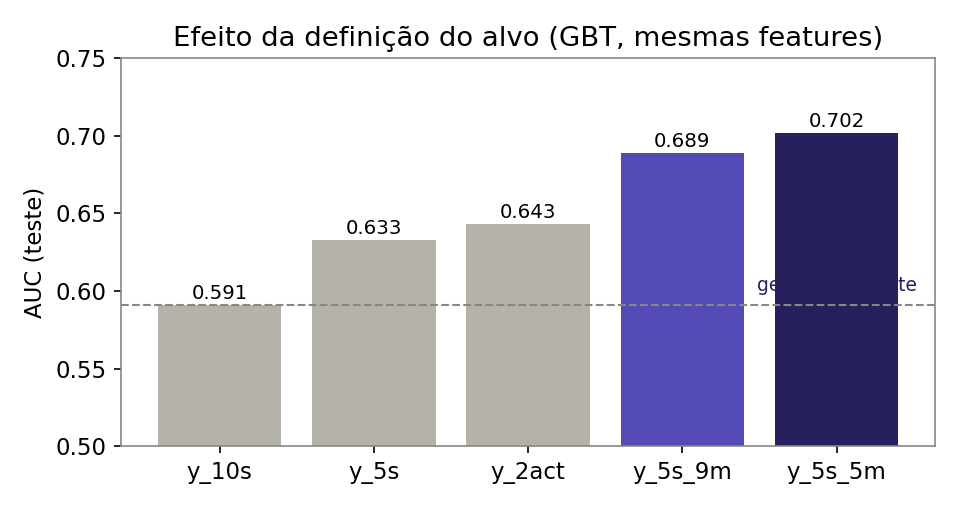
\includegraphics[width=0.72\textwidth]{figs/fig_target.png}
\caption{Efeito da definição do alvo sobre a AUC, com modelo e atributos fixos. Restringir o desfecho no tempo e no espaço é a maior alavanca preditiva.}
\label{fig:target}
\end{figure}

\subsection{Ablação: de onde vem o sinal}
Aplicamos a ablação de atributos (Seção~\ref{sub:ablacao}) aos blocos geometria de jogadores (GEOM), posição em campo (POS) e contexto (CTX). A Figura~\ref{fig:ablation} mostra que, sob \texttt{y\_5s\_5m}, a geometria isolada atinge 0,679 (maior bloco) e contribui $+0{,}071$ marginalmente sobre POS+CTX --- contra $+0{,}053$ sob \texttt{y\_10s}. Ou seja, o alvo restrito não só eleva a AUC: torna a geometria \emph{mais} informativa.

\begin{figure}[ht]
\centering
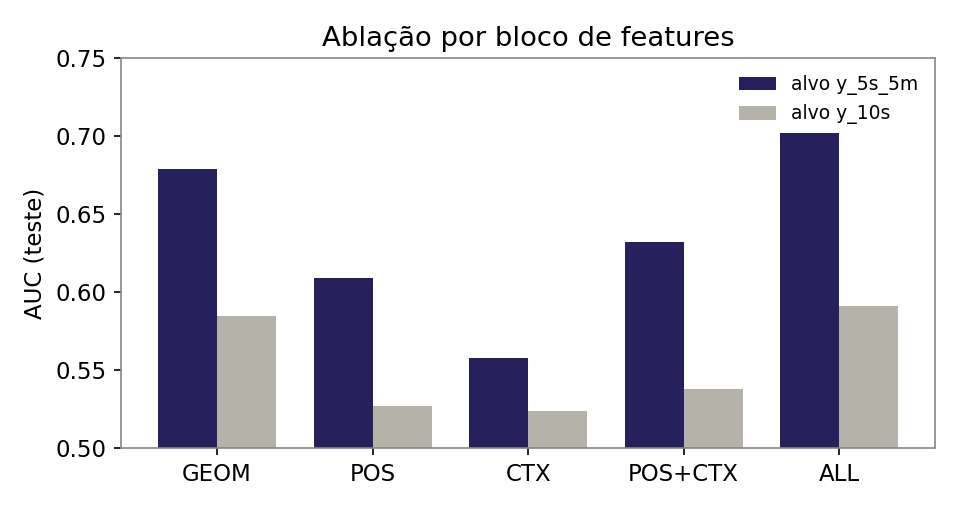
\includegraphics[width=0.72\textwidth]{figs/fig_ablation.png}
\caption{Ablação por bloco de atributos. A geometria de jogadores é o maior contribuinte e ganha importância sob o alvo espacialmente restrito.}
\label{fig:ablation}
\end{figure}

\subsection{Controle: a \emph{base rate} não explica o ganho}
Como \texttt{y\_5s\_5m} tem \emph{base rate} bem menor que \texttt{y\_10s} (6,9\% \emph{vs.}\ 29\%), é preciso descartar que sua AUC maior seja um artefato da prevalência. Conduzimos dois controles sobre o modelo proposto (logística). \textbf{(i) Igualando a \emph{base rate}:} reduzimos por amostragem os positivos do \texttt{y\_10s} até sua base atingir 6,9\% e reajustamos o modelo; a AUC permanece \textbf{0,573} ($\pm$0,007 em 25 repetições), praticamente idêntica à AUC com base cheia (0,571). Baixar a \emph{base rate} \emph{não} eleva a AUC --- coerente com a invariância da ROC-AUC à prevalência. \textbf{(ii) Significância do \emph{gap}:} um \emph{bootstrap} pareado (1.000 reamostragens do mesmo conjunto de teste) da diferença AUC(\texttt{y\_5s\_5m})$-$AUC(\texttt{y\_10s}) resulta em $+0{,}113$, com \textbf{IC\,95\% $[0{,}100;\ 0{,}124]$}, bem acima de zero. O ganho do alvo espacialmente restrito é, portanto, \textbf{real e estatisticamente robusto}, e não um efeito da \emph{base rate} ou da variância amostral.

\subsection{Generalização entre competições}
Para descartar vazamento entre eventos da mesma partida, comparamos o \emph{split} aleatório, o \emph{held-out} da Copa do Mundo 2022 inteira e o \emph{GroupKFold} por partida (alvo \texttt{y\_10s}): 0,591 / 0,590 / 0,590, respectivamente. As estimativas são \textbf{estáveis} --- não há inflação por vazamento.

\section{O modelo proposto: xR logístico calibrado}

\subsection{Logística \emph{vs.} \emph{gradient boosting}}
A Tabela~\ref{tab:usability} compara, sob \texttt{y\_5s\_5m}, uma regressão logística leve e o \emph{gradient boosting} (XGBoost). Para o uso pretendido --- probabilidade/valor esperado em agregado --- a logística é \textbf{tão confiável quanto}, e até marginalmente \emph{melhor calibrada} (ECE 0,002 \emph{vs.} 0,003; Brier praticamente idêntico). O ganho do GBT aparece apenas na discriminação fina (AUC $+0{,}02$, \emph{lift} 2,33$\times$ \emph{vs.} 2,17$\times$), justamente o uso menos confiável. Adotamos a logística como o \textbf{modelo proposto}, por ser leve, interpretável e igualmente calibrada.

\begin{table}[ht]
\centering
\caption{Logística \emph{vs.} \emph{gradient boosting} no alvo \texttt{y\_5s\_5m} (base 6,9\%).}
\label{tab:usability}
\begin{tabular}{lccccccc}
\toprule
Modelo & AUC & PR-AUC & Brier & ECE & Prec.\,top-10\% & \emph{Lift} & Recall\,top-10\% \\
\midrule
Logística (proposto) & 0,683 & 0,124 & 0,063 & \textbf{0,0015} & 0,151 & 2,17$\times$ & 0,217 \\
GBT (XGBoost) & 0,702 & 0,136 & 0,062 & 0,0033 & 0,162 & 2,33$\times$ & 0,233 \\
\bottomrule
\end{tabular}
\end{table}

\subsection{Calibração e curva de ganho}
A Figura~\ref{fig:cal} mostra que o xR é bem calibrado: quando o modelo prevê risco de 20\%, observa-se $\approx$20\%. Essa propriedade legitima o xR como um \emph{expected model}, na mesma linhagem do xG. A Figura~\ref{fig:lift} traduz a discriminação em valor operacional: revisando as 10\% jogadas de maior risco, encontra-se densidade de perdas $2{,}3\times$ maior que o acaso, capturando $\approx$23\% de todas as perdas --- útil para \textbf{triagem de vídeo}, não para alarme automático.

\begin{figure}[ht]
\centering
\begin{minipage}{0.46\textwidth}
\centering
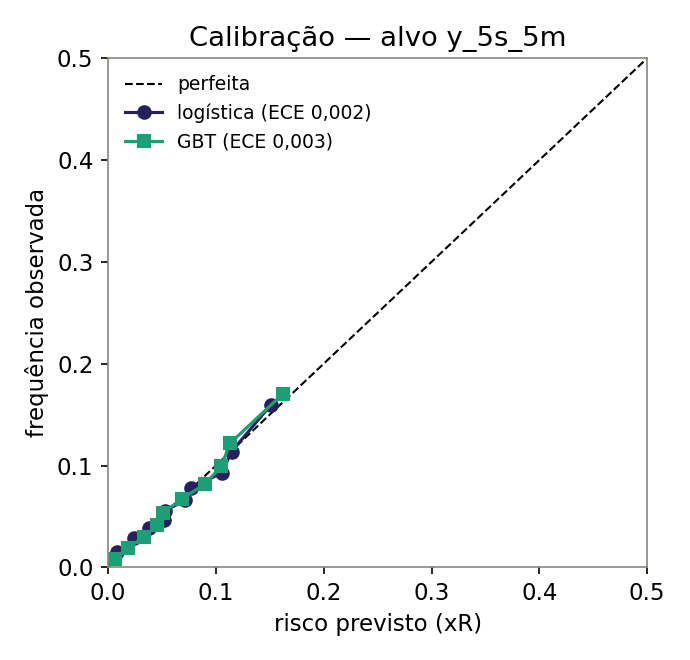
\includegraphics[width=\textwidth]{figs/fig_calibration.png}
\caption{Calibração (\texttt{y\_5s\_5m}): risco previsto \emph{vs.} frequência observada.}
\label{fig:cal}
\end{minipage}\hfill
\begin{minipage}{0.50\textwidth}
\centering
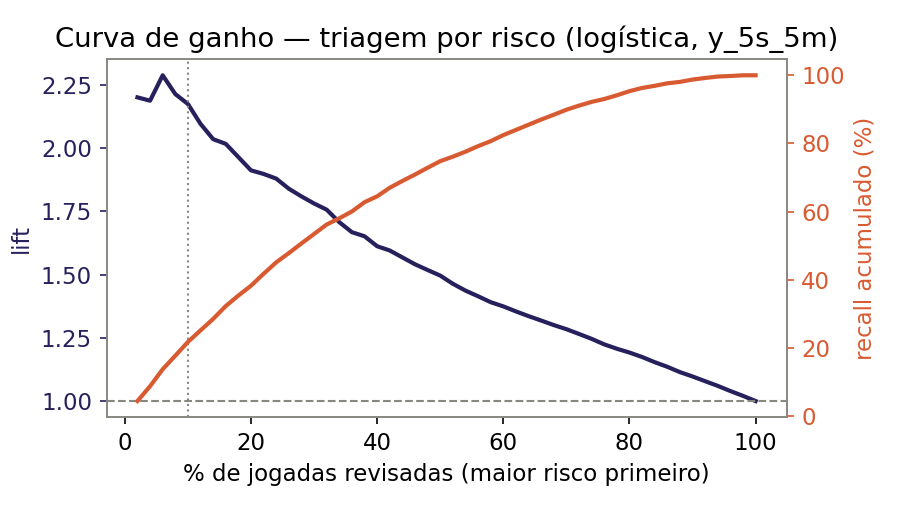
\includegraphics[width=\textwidth]{figs/fig_lift.png}
\caption{Curva de ganho: \emph{lift} e \emph{recall} acumulado por fração revisada.}
\label{fig:lift}
\end{minipage}
\end{figure}

\subsection{Limites de escopo: confiabilidade de \emph{ratings} individuais}
Agregando o desempenho \emph{esperado vs.\ realizado} por jogador, a confiabilidade \emph{split-half} do \emph{rating} de retenção é de apenas \textbf{0,091} (Spearman, 613 jogadores, 91.692 pressões) --- mesmo com a correção de Spearman-Brown ($\approx$0,17), muito abaixo do patamar usável ($\ge$0,5--0,7). A Tabela~\ref{tab:scope} sintetiza: o modelo é apto para uso agregado e calibrado, \textbf{não} para veredito individual de jogada ou de jogador. Esta é uma diferença metodológica central frente a trabalhos que reportam \emph{rankings} individuais sem auditoria.

\begin{table}[ht]
\centering
\caption{Aptidão por uso. Calibração habilita o agregado; baixa confiabilidade impede o individual.}
\label{tab:scope}
\begin{tabular}{lcc}
\toprule
Uso pretendido & Evidência & Apto? \\
\midrule
Probabilidade / valor esperado (agregado) & ECE 0,003; Brier 0,062 & Sim \\
Triagem de vídeo / priorização & \emph{lift} 2,3$\times$ (top-10\%) & Sim (apoio) \\
Alerta de jogada isolada & $\approx$84\% falso alarme & Não \\
\emph{Rating} individual de jogador & confiabilidade 0,09 & Não \\
\bottomrule
\end{tabular}
\end{table}

\section{Aplicação prática}

A Figura~\ref{fig:flow} resume o fluxo de uso do xR por uma equipe de analistas e comissão técnica. Após cada jogo, o modelo pontua toda pressão; os xR sobem de jogada para \textbf{zona, gatilho e time}, onde a leitura é confiável. As aplicações naturais são: \emph{(i)} \textbf{análise de adversário} (onde e como o próximo oponente recupera/perde a bola, alimentando o plano de pressing); \emph{(ii)} \textbf{treino} (desenho de gatilhos a partir de padrões esperados \emph{vs.} realizados); \emph{(iii)} \textbf{scouting} (métricas agregadas com amostra grande, cruzadas com observação); e \emph{(iv)} \textbf{revisão pós-jogo}, comparando o xR esperado com o que de fato aconteceu e priorizando os clipes de maior discrepância. Em todas as etapas, o modelo \emph{sugere}; o analista contextualiza com vídeo; a comissão técnica decide.

\begin{figure}[ht]
\centering
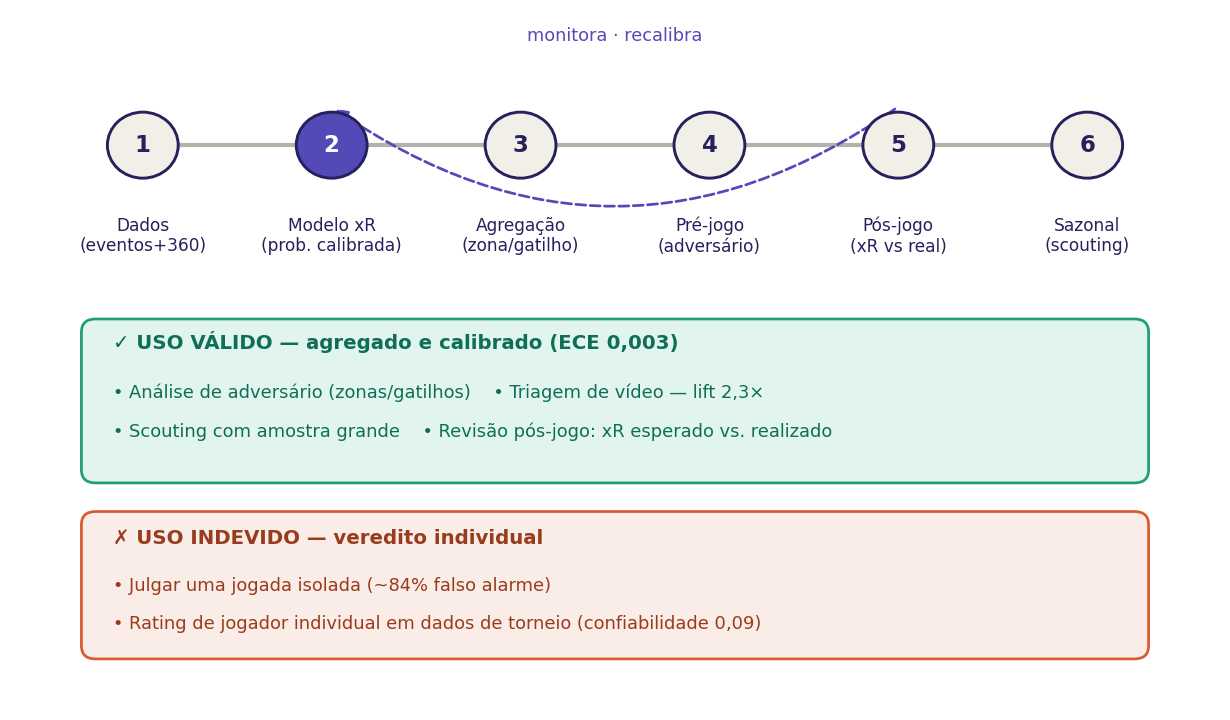
\includegraphics[width=0.92\textwidth]{figs/fig_flow.png}
\caption{Fluxo de aplicação do xR e delimitação de escopo (verde: uso válido e calibrado; vermelho: fora do escopo).}
\label{fig:flow}
\end{figure}

\section{Conclusão}

Apresentamos o xR, um modelo logístico calibrado de recuperação esperada sob pressão. O resultado mais importante é metodológico: a \textbf{definição do alvo} --- e não a sofisticação do modelo --- determina a previsibilidade e o quanto a geometria dos jogadores carrega sinal; um alvo espacialmente restrito eleva a AUC de 0,59 para 0,70 e torna a geometria mais informativa. Um modelo leve e interpretável basta para o uso que importa na ponta: análise de adversário, treino, \emph{scouting} e revisão pós-jogo, sempre em agregado e com probabilidades calibradas. Delimitamos o escopo com evidência: \emph{ratings} individuais de jogador não são confiáveis no volume de dados de torneios. Como trabalho futuro, destacam-se a ponderação por valor (xT/VAEP) do risco de perda, formulações de sobrevivência para o horizonte temporal, e a validação externa dos \emph{ratings} com dados de temporada completa.

~\\
\bibliographystyle{sbpo}
\bibliography{artigo-xR}

\end{document}
